\documentclass{article}

\usepackage[a4paper, total={6in, 8in}]{geometry}
\usepackage[utf8]{inputenc}
\usepackage{amsmath}
\usepackage{amssymb}
\usepackage{amsthm}
\usepackage{fancyhdr}
\usepackage{enumitem}
\usepackage[makeroom]{cancel}
\usepackage{graphicx}

\pagestyle{fancy}
\fancyhf{}
\lhead{John J Li}
\rhead{MAT300 Project Paper}
\rfoot{\thepage}
\lfoot{April 2021}
\renewcommand{\headrulewidth}{0.4pt}
\renewcommand{\footrulewidth}{0.4pt}

\setlength{\parskip}{1em}
\setlength\parindent{0px}
\title{MAT300 Project Paper}
\date{\today}
\author{John J Li}

\begin{document}
    \maketitle
    \thispagestyle{empty}

    %###################################################################################

    \section*{Problem 1}

    Show that $\forall_x P(x)\lor \forall_x Q(x)$ is not always equivalent to $\forall_x (P(x)\lor Q(x))$. On the other hand, show that $\forall_x P(x) \lor \forall_x Q(x)$ is logically equivalent to $\forall_x\forall_y (P(x)\lor Q(y))$. (Domains for x and y are the same). You should also compare these two statements to better explain why they differ.
    \begin{proof}
        We will show that $\forall_x P(x)\lor \forall_x Q(x)$ is not always equivalent to $\forall_x (P(x)\lor Q(x))$. Suppose $P(x)$ means "x lives in the ocean" and $Q(x)$ means "x lives on land". Then $\forall_x P(x)\lor \forall_x Q(x)$ would mean "all of x lives in the ocean or all of x lives on land" whereas $\forall_x(P(x)\lor Q(x))$ would mean "all of x lives in the ocean or on land". Now consider three animals in $x$, a seal (lives in the ocean and on land), a bear (lives on land but not in the ocean), and a whale (lives in the ocean but not on land). Then it is true that all three animals lives in the ocean or on land but it is false to say all three animals lives in the ocean or all three animals lives on land. Thus $\forall_x P(x)\lor \forall_x Q(x)$ is not always equivalent to $\forall_x (P(x)\lor Q(x))$.
    \end{proof}
    \begin{proof}
        We will show that $\forall_x P(x) \lor \forall_x Q(x)$
        is logically equivalent to $\forall_x\forall_y (P(x)\lor Q(y))$. Suppose $x,y$ are in the same domain.

        Case 1: Suppose $\forall_x P(x) \lor \forall_x Q(x)$, we will show 
        $\forall_x\forall_y (P(x)\lor Q(y))$.

        Let $\forall_x P(x)\lor\forall_x Q(x)$ represent different statements on two sets $x,y$ which have the same domain. Then it can be said that $\forall_x P(x) = P(x_1)\land P(x_2) \land ... P(x_n)$ and $\forall_y Q(y) = Q(y_1)\land Q(y_2)\land ... Q(y_n)$ where $n$ is the number of elements in $x,y$.
        Then we have $P(x_1)\land P(x_2) \land ... P(x_n)\lor Q(y_1)\land Q(y_2)\land ... Q(y_n)$. Which is the same as $\forall_x\forall_y (P(x)\lor Q(y))$.

        Case 2: Suppose $\forall_x\forall_y (P(x)\lor Q(y))$, we will show 
        $\forall_x P(x) \lor \forall_x Q(x)$.

        We can write $\forall_x P(x) \lor \forall_x Q(x)$ as $P(x_1)\land P(x_2) \land ... P(x_n)\lor Q(y_1)\land Q(y_2)\land ... Q(y_n)$ where $n$ is the number of elements in $x,y$. This is also $\forall_x P(x) = P(x_1)\land P(x_2) \land ... P(x_n)$ and $\forall_y Q(y) = Q(y_1)\land Q(y_2)\land ... Q(y_n)$.
        And it can be written as $\forall_x P(x)\lor\forall_y Q(y)$. Since it is assumed $x,y$ are in the same domain we can subsitute $y$ for $x$ to get $\forall_x P(x)\lor\forall_x Q(x)$.

        Thus $\forall_x P(x) \lor \forall_x Q(x)$
        is logically equivalent to $\forall_x\forall_y (P(x)\lor Q(y))$.

    \end{proof}


    %###################################################################################

    \section*{Problem 2}

    A celebrity at a party is a guest who is known by every other guest at the party but doesn't know any of them.

    (a) Show that if there are $n\geq 1$ guests at a party, then you can identify the celebrity (if one exists) by asking at most $3(n-1)$ questions, each question consists of asking person $A$ if he (or she) knows person $B$ (to which you will obtain a truthful yes/no answer).

    \begin{proof}
        Suppose there are an arbitrary number $n\geq 1$ guests at a party and there may or may not be a celebrity at the party. Assume all guests knows the celebrity but the celebrity knows no one. Assume each guest will give a honest true or false answer when they are asked if they know another guest. We will prove that the celebrity can be identified by asking at most $3(n-1)$ questions.
        
        If $n=1$ then that guest is the celebrity (by definition) and you do not need to ask any questions; thus $0\leq 3(n-1)$.
        
        Else, suppose each guest is an element of a set; traverse the set by asking each guest whether or not they know all other guests in the set. If a guest says they do not know a guest, you remove the known guest from the set (for example, if guest A doesn't know guest B, you remove guest B from the set). Continue with the questioning until either a guest says they know another guest or there is one remaining guest. If a guest knows another guest then remove the guest you were questioning (for example, if guest A knows guest C, remove guest A from the set). If there is one remaining guest, then you would've asked $n-1$ questions since you are able to eliminate a guest for each question asked except for one. 

        The remaining guest is either a celebrity or there are no celebrities at the party. To know if the remaining guest is a celebrity or not, ask each guest that is not the remaining guest if they know the remianing guest. If all guests knows the remaining guest, then the remaining guest is a celebrity, if a guests doesn't know the remaining guest then the remaining guest is not a celebrity and the questioning may end. You would've asked at most $n-1$ questions since you dont need to ask the remaining guest.

        Since you must iterate over the initial set of guests twice with each iteration asking $n-1$ questions, the maximum number of questions you need to ask is $2(n-1)\leq 3(n-1)$.
    \end{proof}

    (b) How many questions suffice if it's known that celebrity is attending a party?

    Suppose a celebrity is attending the party of an arbritray number $n\geq 1$ guests. Then $n-1$ questions will suffice to identify the celebrity. Look to the proof from (a), you will only need to iterate over the initial set of guests once since you do not need to check that every guest knows the remaining guest.


    %###################################################################################

    \section*{Problem 3}

    Let $B$ be the 8 by 8 chessboard with one black and white square removed. Show that it is possible to tile $B$ with domino pieces.

    \begin{proof}
        Let $B$ be the 8 by 8 chessboard with one black and white square removed. We will show that it is possible to tile $B$ with domino pieces.

        \begin{figure}[ht]
            \centering
            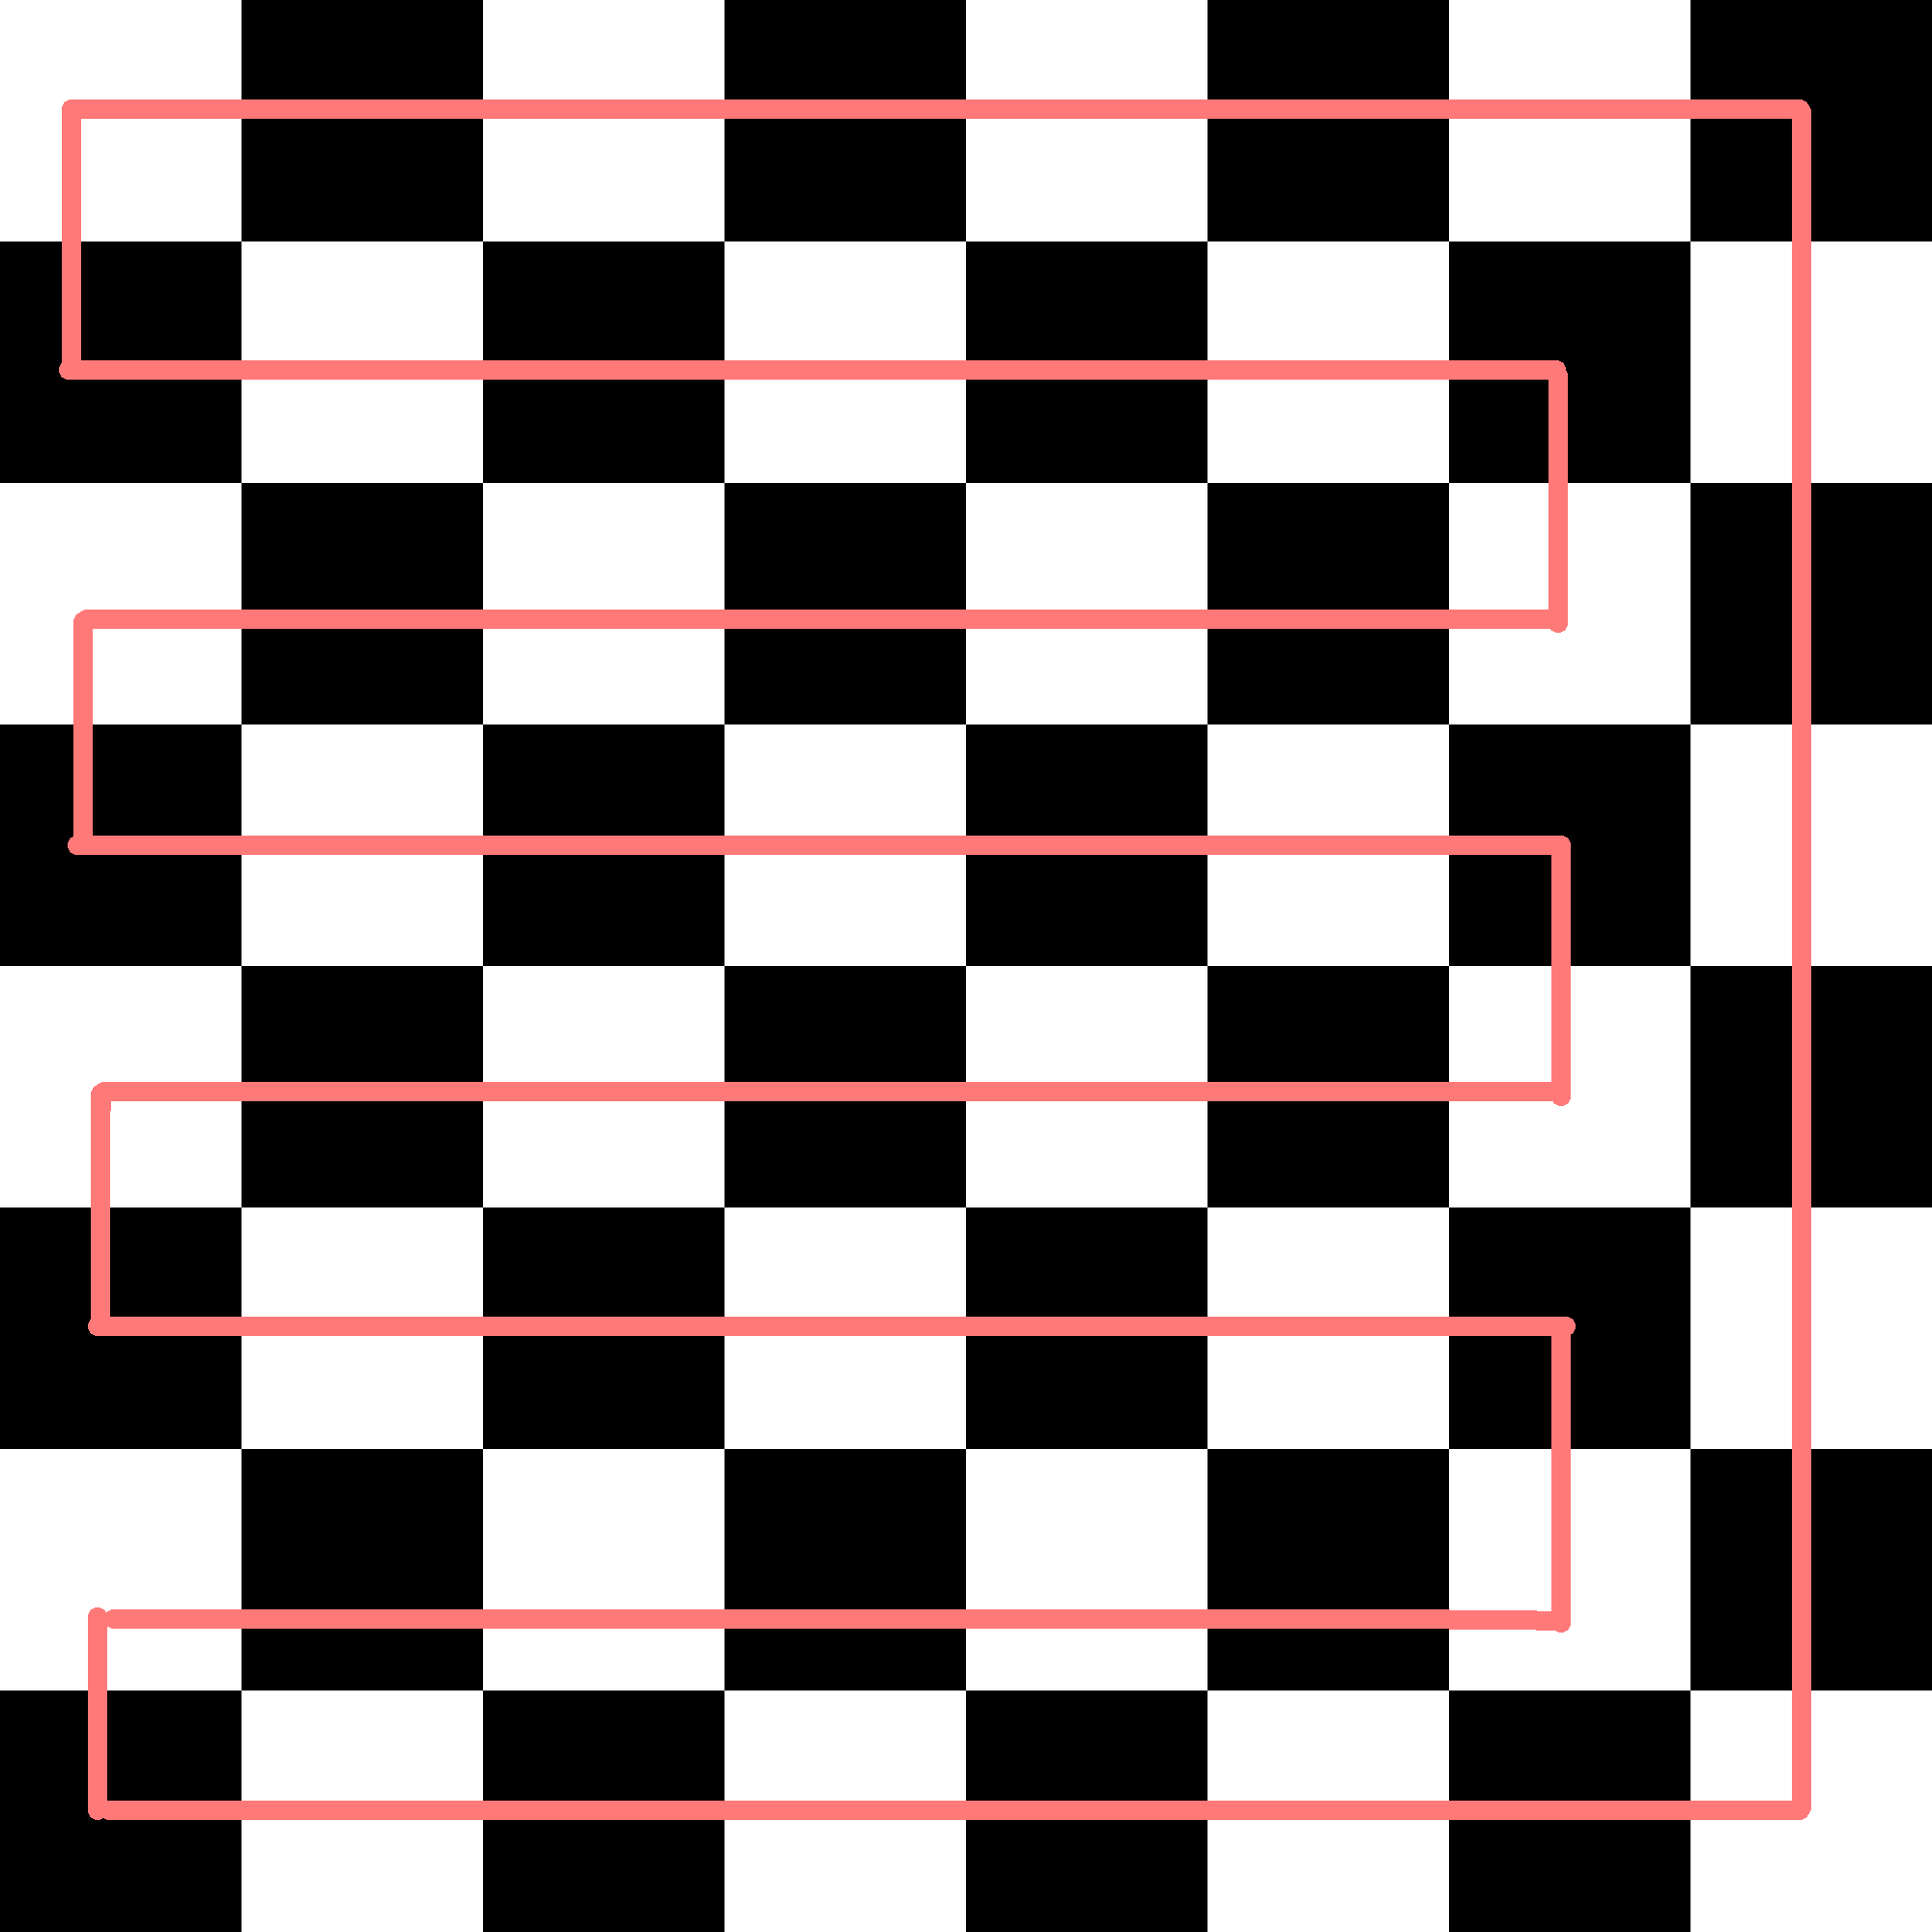
\includegraphics[width=0.25\textwidth]{Q3_01.png}
            \caption{Chessboard with length of pink rope stretching across every tile}
            \label{fig:rope1}
        \end{figure}
        \begin{figure}[ht]
            \centering
            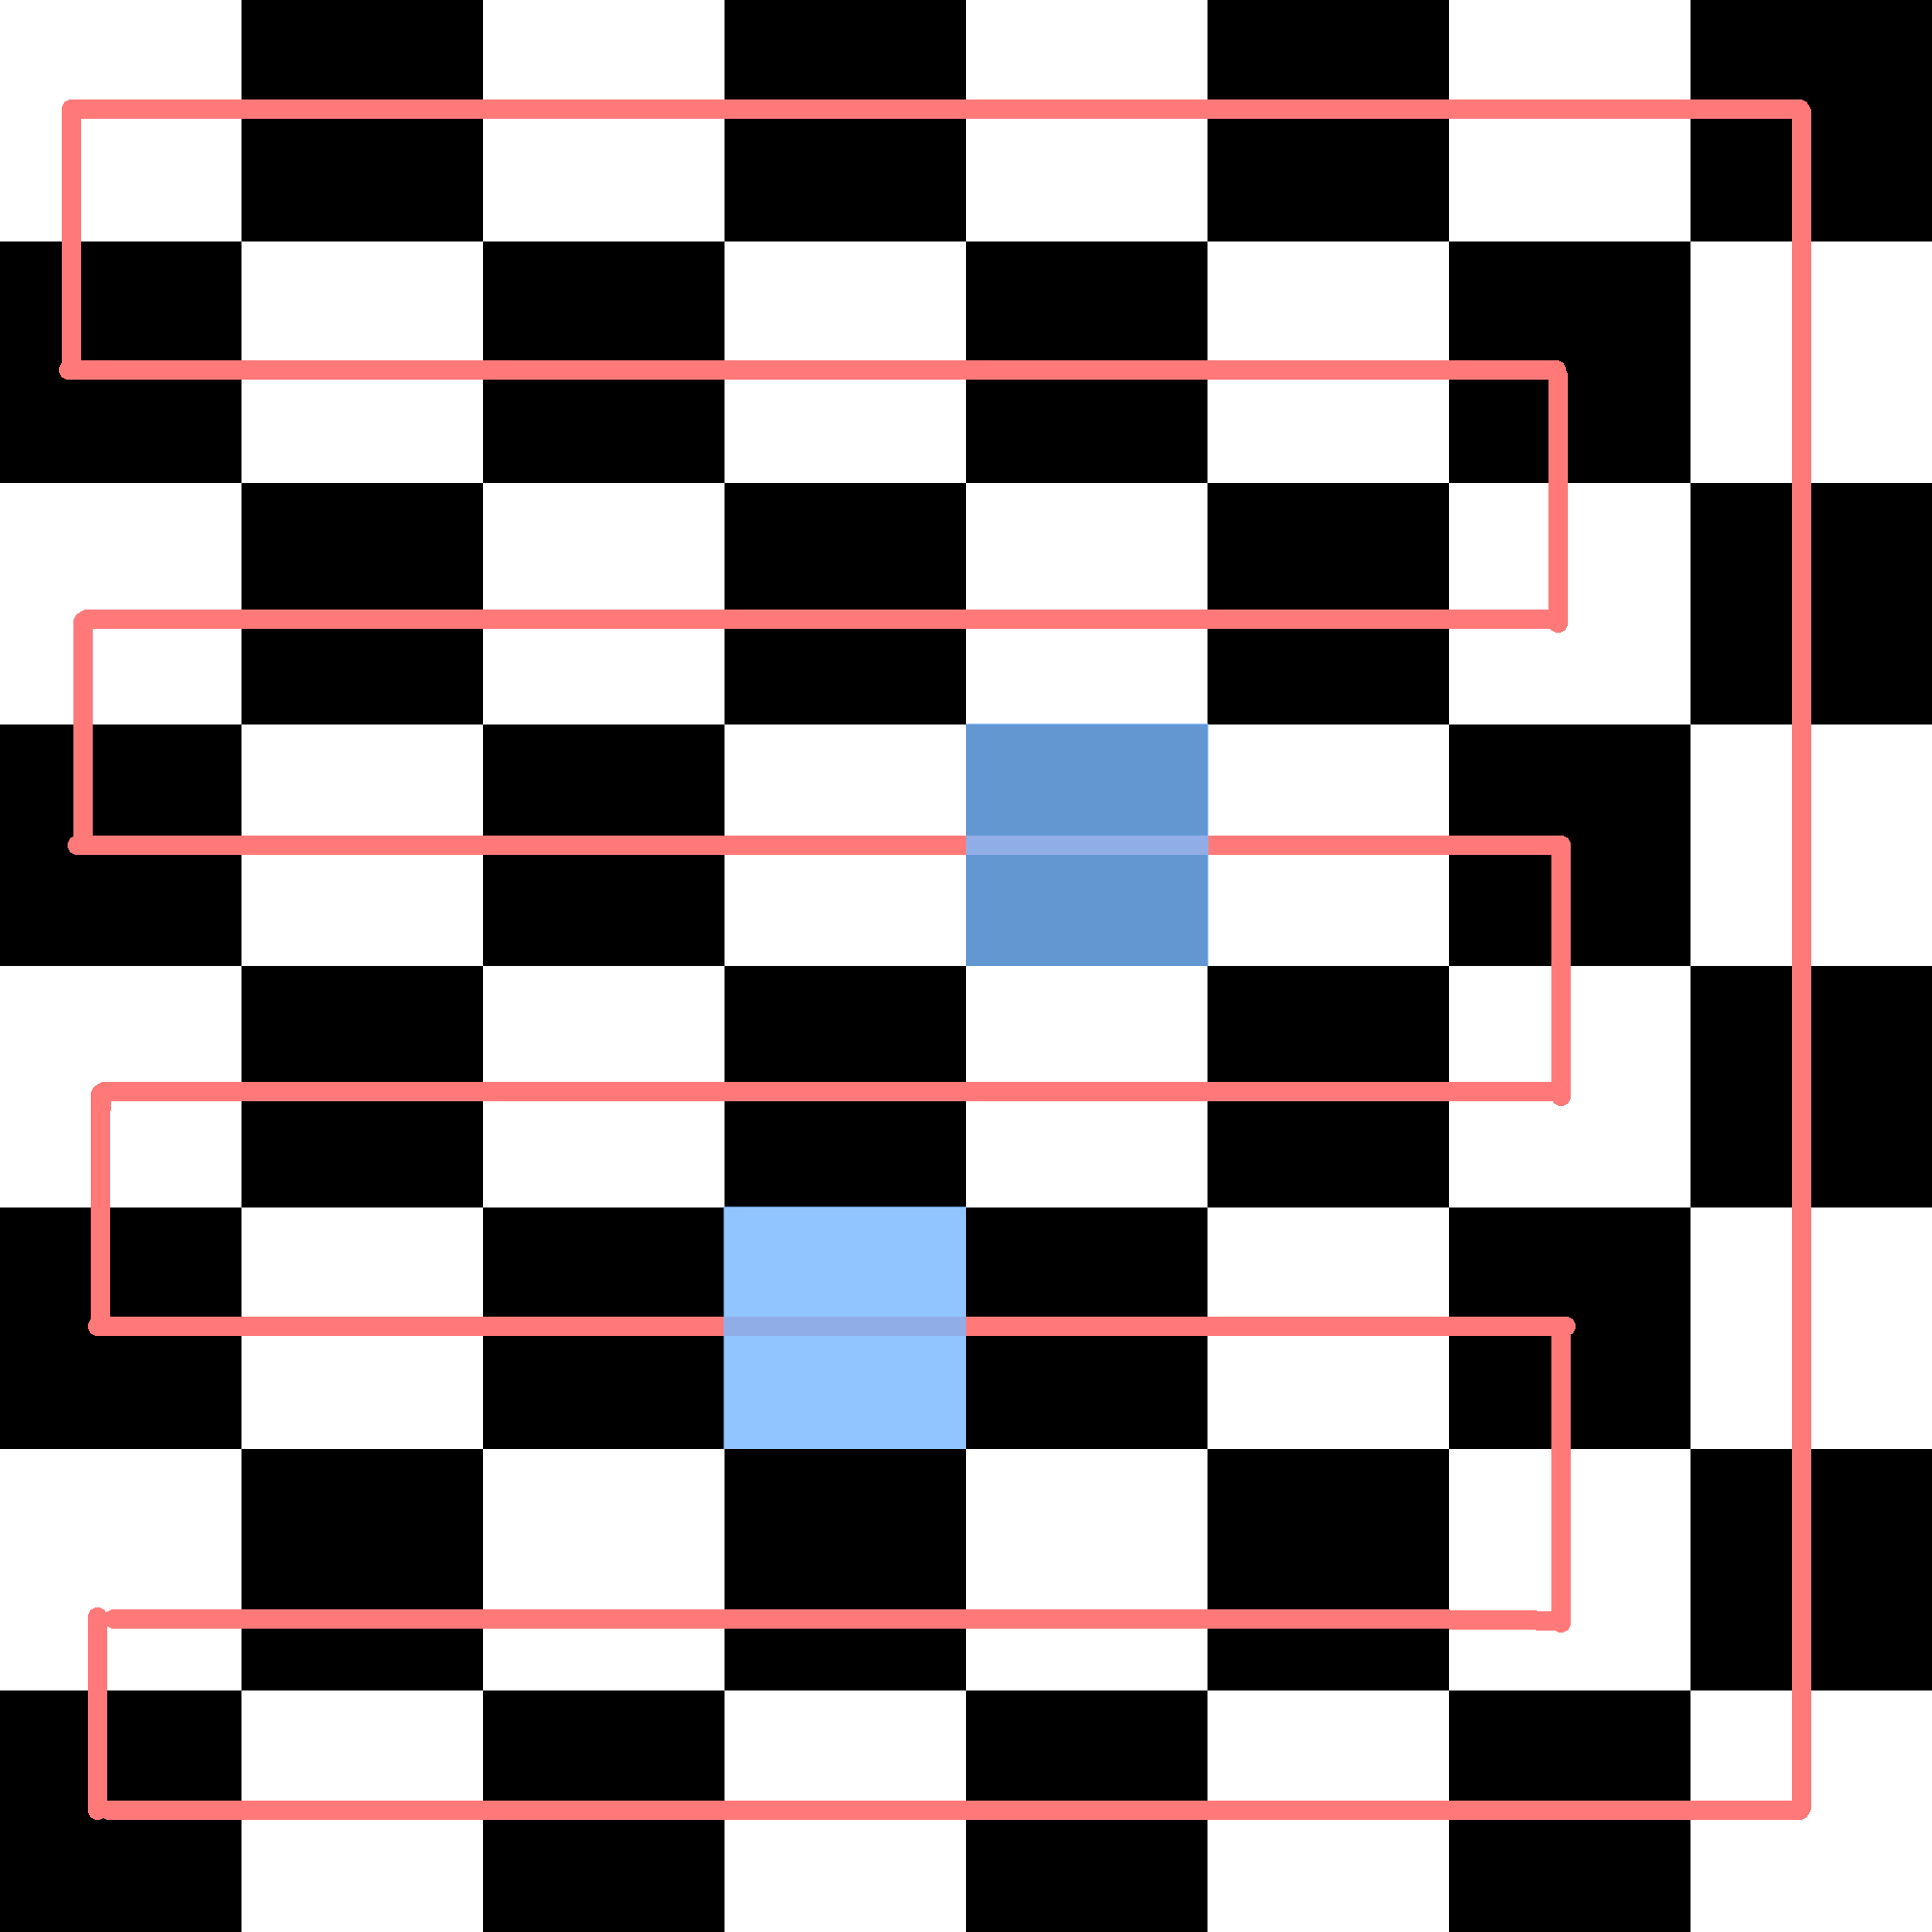
\includegraphics[width=0.25\textwidth]{Q3_02.png}  
            \caption{Chessboard with length of rope and one black and white tile removed}
            \label{fig:rope2}
        \end{figure}

        Now suppose a rope stretched across the chessboard, connecting each square to each other shown in figure \ref{fig:rope1}. And suppose a black and a white square is removed along with the section of rope on top of them. Then since black and white squares are alternating, the length of ropes between them is always even. And it is possible to tile an even number of tiles with dominos.
    \end{proof}


    %###################################################################################

    \section*{Problem 4}

    Mike and Barbara go to a dinner with $n$ other couples. Each person shakes
    hands with everyone she or he doesn't know. Later, Mike discovers that
    each of the remaining $2n + 1$ people shook hand with a different number
    of people. How many people did Barbara shake hands with? (Prove your
    claims.)

    Barbara shook hands with $n$ people. 

    \begin{proof}
        Suppose Mike and Barbara goes to dinner with $n$ others couples and each person shakes hands with everyone he or she doesn't know. Suppose Mike discovers that each remaining $2n+1$ people shook hands with a different number of people. We will show Barabara shook hands with $n$ people.

        Since we know Mike heard that everyone shook hands with a different amount of people, we know (1) Mike shook hand with the same amount of people as someone else, and (2) the number of hands two people shook adds up to $2n$.

        Suppose there is a set of size $2n+1$, containing each person at the dinner and Barbara. Thus, each person in the set shook hands with $\{0,1,2,...,2n\}$ people and each person in the set shook an unique number of hands. Suppose we took the person who shook $2n$ hands and removed everyone that person shook hands with from the set. Then in the original set, we have two people, the person who shook $2n$ hands and the person who shook $0$; since everyone else shook hands with at least one person, these two people must be a couple. Then we group everyone who isn't in the first set into a new set and removing everyone that the next highest handshaker that shaken hands with. Since the next highest handshaker didn't shake hands with their spouse and the person who shook $0$ hands, the only two people in the next set would be the next highest handshaker and their spouse. By continuing this pattern, we have a set of size $n$ subsets that each contains a couple except for the last subset which only contains Barbara.

        This means Barbara shook the median number of hands which is $\frac{2n}{2} = n$.
    \end{proof}
\end{document}